\documentclass[tikz,border=3pt]{standalone}
\usepackage{amsmath,amssymb}
\usetikzlibrary{calc}
\begin{document}
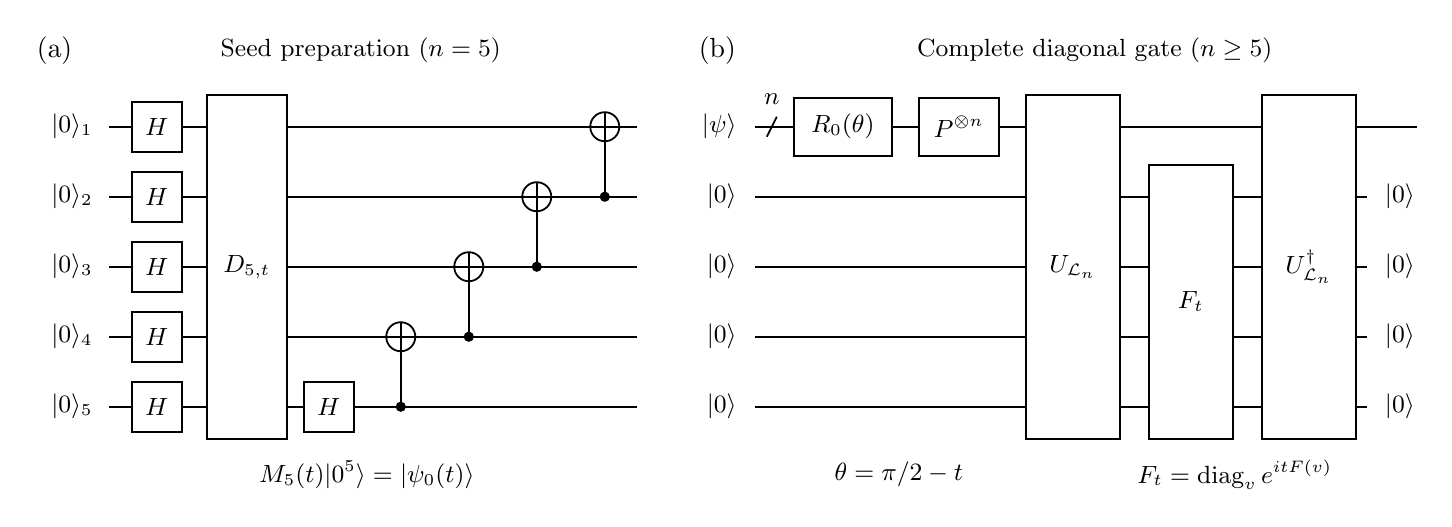
\begin{tikzpicture}[x=1in,y=1in,
  line width=0.65pt,
  every node/.style={font=\fontsize{9}{11}\selectfont},
  gate/.style={draw,fill=white,minimum width=0.25in,minimum height=0.25in,inner sep=0pt},
  multigate/.style={draw,fill=white,inner sep=0pt},
  control/.style={circle,fill=black,inner sep=0pt,minimum size=3.7pt},
  target/.style={circle,draw,fill=white,inner sep=0pt,minimum size=10.5pt}]

% 左图：门按从左至右的时间顺序绘制。
\node[anchor=west,font=\fontsize{10}{12}\selectfont] at (0.02,2.08) {(a)};
\node at (1.69,2.08) {Seed preparation ($n=5$)};
\foreach \j/\y in {1/1.70,2/1.35,3/1.00,4/0.65,5/0.30}{
  \node[anchor=east] at (0.40,\y) {$|0\rangle_{\j}$};
  \draw (0.43,\y) -- (3.07,\y);
  \node[gate] at (0.67,\y) {$H$};
}
\node[multigate,minimum width=0.40in,minimum height=1.72in] at (1.12,1.00) {$D_{5,t}$};
\node[gate] at (1.53,0.30) {$H$};
\foreach \x/\yc/\yt in {1.89/0.30/0.65,2.23/0.65/1.00,2.57/1.00/1.35,2.91/1.35/1.70}{
  \draw (\x,\yc) -- (\x,\yt);
  \node[control] at (\x,\yc) {};
  \node[target] at (\x,\yt) {};
  \draw (\x-0.073,\yt) -- (\x+0.073,\yt);
  \draw (\x,\yt-0.073) -- (\x,\yt+0.073);
}
\node at (1.72,-0.04) {$M_5(t)|0^5\rangle=|\psi_0(t)\rangle$};

% 右图：一根 n 位数据线，四根初始化并恢复为零的辅助位。
\node[anchor=west,font=\fontsize{10}{12}\selectfont] at (3.33,2.08) {(b)};
\node at (5.36,2.08) {Complete diagonal gate ($n\geq5$)};
\node[anchor=east] at (3.62,1.70) {$|\psi\rangle$};
\draw (3.66,1.70) -- (6.97,1.70);
\draw (3.72,1.65) -- (3.77,1.75);
\node[anchor=south] at (3.745,1.76) {$n$};
\foreach \y in {1.35,1.00,0.65,0.30}{
  \node[anchor=east] at (3.62,\y) {$|0\rangle$};
  \draw (3.66,\y) -- (6.72,\y);
  \node[anchor=west] at (6.76,\y) {$|0\rangle$};
}
\node[gate,minimum width=0.49in,minimum height=0.29in] at (4.10,1.70) {$R_0(\theta)$};
\node[gate,minimum width=0.40in,minimum height=0.29in] at (4.68,1.70) {$P^{\otimes n}$};
\node[multigate,minimum width=0.47in,minimum height=1.72in] at (5.25,1.00) {$U_{\mathcal L_n}$};
\node[multigate,minimum width=0.42in,minimum height=1.37in] at (5.84,0.825) {$F_t$};
\node[multigate,minimum width=0.47in,minimum height=1.72in] at (6.43,1.00) {$U_{\mathcal L_n}^{\dagger}$};
\node at (4.38,-0.04) {$\theta=\pi/2-t$};
\node at (6.06,-0.04) {$F_t=\operatorname{diag}_{v}e^{itF(v)}$};
\end{tikzpicture}
\end{document}
